% !TEX encoding = UTF-8 Unicode
% !TEX TS-program = xelatex

\documentclass[11pt]{article}
\usepackage{fontspec}
\defaultfontfeatures{Mapping=tex-text}
\usepackage{xunicode}
\usepackage{xltxtra}
\usepackage{verbatim}
\usepackage[margin= 1 in]{geometry} % see geometry.pdf on how to lay out the page. There's lots.
\geometry{letterpaper} % or letter or a5paper or ... etc
%\usepackage[parfill]{parskip}    % Activate to begin paragraphs with an empty line rather than an indent 
\usepackage{mathrsfs}
\usepackage{bbding}
\usepackage[usenames,dvipsnames]{color}
\usepackage{natbib}
\usepackage{stmaryrd}
%\usepackage{mathpartir}
\usepackage{txfonts}
\usepackage{graphicx}
\usepackage{fullpage}
\usepackage{hyperref}
\usepackage{amssymb}
\usepackage{epstopdf}
\usepackage{fontspec}
%\setmainfont{Hoefler Text}
\setmainfont[BoldFont={Minion Pro Bold}]{Minion Pro}
\usepackage{hyperref}
\usepackage{lastpage, fancyhdr}
%\usepackage{setspace}
\pagestyle{fancy}
\lhead{}
\chead{Lecture 8, Plato's \emph{Meno} continued\space---\space Handout} 
\rhead{}
\lfoot{}
\cfoot{\thepage\space of \pageref{LastPage}} 
\rfoot{}
\footskip=30 pt
\headsep=20pt
\thispagestyle{empty}
\hypersetup{colorlinks=true, linkcolor=Sepia, urlcolor=Sepia, citecolor=BrickRed}
\DeclareGraphicsRule{.tif}{png}{.png}{`convert #1 `dirname #1`/`basename #1 .tif`.png}
\usepackage{polyglossia}
\setdefaultlanguage{english}
\setotherlanguage{greek}
\newfontfamily\greekfont{Gentium Plus}
\newcommand{\gk}[1]{\textgreek{#1}}
\newcommand{\gloss}[1]{(\textgreek{#1})}

\usepackage{covington}
\usepackage{fixltx2e}
\usepackage{graphicx}
\begin{document}

%\maketitle
\thispagestyle{empty}
\begin{center} \LARGE{PHIL 321\\ Lecture 8: Plato's \emph{Meno} continued}\\ \vspace*{2mm}
\large{9/24/2013}\end{center}
\thispagestyle{empty}\vspace*{3mm}
\vspace*{-8mm}

\section*{Recollection revisited}

\noindent [1] The slave is said to have no geometrical knowledge before the discussion (85e)
\vspace*{2mm}

\noindent [2] S claims that he has not taught the slave anything during their discussion
\begin{itemize}\item{S is probably working with a conception of ``teaching'' on which for S to teach X that P would be for X to come to believe that P \emph{only because} S tells X that P}\end{itemize}

\noindent [3] But, by the end of the discussion, the slave has the opinion that the double-area square comes to be from the diagonal of the original square

\begin{itemize}\item{So, given [2], S asks where that opinion came from}\item{S claims that it must have been, in some sense, in the slave already (85c)}\end{itemize}

\noindent [4] S claims that the slave, at the end of the discussion, does not yet have \emph{epist\^{e}m\^{e}} of the geometrical fact, but that the slave \emph{will} acquire it through further questioning (85c7-d4)
\vspace*{2mm}

\noindent [5] Since that further questioning will not violate [2], S concludes that the slave will acquire the knowledge ``from himself by himself''
\vspace*{2mm}

\noindent [6] The phenomenon described in [5] is claimed to be an instance of ``recollection'' (\emph{anamn\^{e}sis})
\vspace*{2mm}

\noindent So, S takes himself to have answered the paradox of inquiry by showing that the slave can go from a state of not having \emph{epist\^{e}m\^{e}} (at least, not explicitly) to a state of having \emph{epist\^{e}m\^{e}} (i.e. explicitly). And, he maintains that it is because the slave once knew, then forgot, and through questioning can be made to recollect, that successful inquiry is possible. So, is it because those who don't know have true opinions which they can systematize in some way that successful inquiry is possible?
\vspace*{2mm}

\noindent Important question: Even if we grant [1]-[4] do we have to think that the slave has (or, will have) recollected knowledge? What alternative explanations for the success of the slave's discussion might we consider?

\section*{The scope of recollection}

\noindent What kinds of truths does S think we can recollect?

\begin{itemize}\item{He clearly allows geometrical truths (and so mathematical truths generally?). He should allow ethical truths (including truths about value) (otherwise the unity of the dialogue would be in jeopardy). He also suggests nature ``as a whole''?---What could that mean?}\item{What about empirical truths?}\end{itemize}

\section*{Is virtue knowledge/understanding?}

\noindent After the exchange, M insists that S address whether virtue is teachable, despite S's demand to determine what virtue is first
\vspace*{2mm}

\noindent S again refuses to address that question directly, but instead notes that if virtue is knowledge, then virtue will be teachable (and if virtue is not knowledge, it will not be teachable)
\vspace*{2mm}

\noindent So he then turns his attention to the question whether virtue is knowledge, considering arguments for and against
\begin{itemize}\item{The main \emph{pro} argument is that, since virtue is beneficial, and all actions guided by knowledge turn out well, virtue must be knowledge}\end{itemize}

\section*{The difference between true belief/opinion and knowledge/understanding}

\noindent S maintains that they were right to say that actions guided by knowledge always turn out correctly, BUT
\vspace*{2mm}

\noindent They were wrong to say that \emph{only} actions guided by knowledge turn out correctly---actions guided by true opinion (\emph{doxa}) also turn out correctly

\begin{itemize}\item{The example of the ``Road to Larissa'' (97a5-c2) is supposed to show this}\end{itemize}

\noindent This leads M to ask ``why knowledge (\emph{epist\^{e}m\^{e}}) is prized far more highly than right opinion, and why they are different'' (97d1-2)
\vspace*{2mm}

\noindent S answers that right opinion is ``upgraded'' into knowledge by a ``giving an account of the reason why'' (i.e. by working out the explanation of the relevant fact) which ``ties'' the opinion to the soul. Knowledge is more valuable because it remains in place.
\vspace*{2mm}

\noindent Question: What has \emph{not} been done in the discussion with the slave such that further questioning could lead the slave to work out the explanation of the geometrical theorem?
\vspace*{2mm}

\section*{How natures can play an explanatory role}

\noindent Euclid's \emph{Elements} Book 1, Proposition 34: In parallelogrammic figures the opposite sides and angles are equal to one another, and \emph{a diagonal cuts them in half}
\vspace*{2mm}

\noindent And, [F1] since the point A is the center of the circle CDB, [F2] AC is equal to AB.

\begin{figure}[h!]
\centering
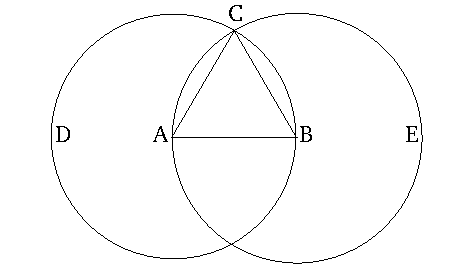
\includegraphics[scale=0.7]{circle}
%\caption{}
%\label{fig:prop 34}
\end{figure}

\noindent Definition of Circle: A Circle is a plane figure contained by one line, such that all of the straight-lines falling upon it from one point among those lying within the figure are equal to one another

\end{document}
